\section{Experiments and Results}
Description generall
limiations of work
\subsection{Extending the network}
The first experiment makes use of network extension to see wether the network splits.
The base network for the extension is a (4, 8, 8, 2) network. 
It has 112 weights, which is also the pruning target.
The base network is trained without pruning, since it is already at the pruning target.
The network is extended up until 20 levels.
The final network has a shape of (4, 1310, 1310, 2) and 1000000? prunable parameters before pruning.
The pruning rate is fixed to $p=0.32$.

The Iterative Magnitude Pruning workflow is executed at every extension level, creating 20 runs.

INSERT A TABLE OF THE PRUNING TRAJECTORIES 
0, 
0, 1
0, 1, 2 and so on 

The number of pruning levels increases by one for each network extension.
Note that the pruning trajectories overlap.
Each network goes through the same number of parameters as the network it was extended from plus one additional step in the beginning.

There are four different scenarios that can happen:
\begin{enumerate}
    \item split (and not degrade) \\
    The network splits at some point and keeps all input and output nodes until after the last pruning level 
    \item split and degrade \\
    The network splits at some point and has all input and output nodes.
    At a later iteration, the network degrades( it loses at least one input or output)
    \item not split but degrade \\
    The network degrades before a split happens
    \item not split and not degrage \\
    The network does neither split, nor degrade. 
    The result is a single network that contains all input and output nodes of all tasks.
\end{enumerate}

For extension levels 0 to 6, where the network has a shape of (4, 31, 31, 2), the network did not seperate into disconnected subnetworks.
The first time the network seperates is at 7 extension levels. 
The network has a shape of (4,38,38,2) and is pruned 7 times.
Though only one out of four runs succesfully split the network, after the 8th extension level, the network consistently and reliably seperates.
 
Only after extending the network 12 times to a shape of (4, 104, 104, 2) the first network degrades after having seperated.
This effect occurs more often the more pruning levels are done.
One possible explanation that the final number of active weights in the network correlates with the number of pruning iterations.
If there are more pruning iterations, the final network contains less active weights, making it more likely to degrade.

\begin{figure}[ht]
    \centering
    \includegraphics[width=1.0\linewidth]{collateral-damage.png}
    \caption{
        The figure depicts the number of active weights after the last pruning iteration of extended networks.
        On the x-axis, the hidden dimension of the neural network is displayed.
        On the y-axis, the number of active weights.
        A clear pattern emerges, showing a correlation between number of pruning iterations and the number of active weights in the final network.
    }
    \label{fig:collateral_damage}
\end{figure}

Interestingly, the network first splits with $7$ pruning levels and a shape of (4,38,38,2).
Afterwards, the network consistently splits.

The question arises for what the main driver for splitting in this case is.
The model size or the number of pruning iterations.
To get a first impression and intuition about this question, a tangential experiment was launched with a grid of parameters.
Four different network sizes and six different values for the number of pruning iterations are used, and each experiment is repeated four times with different seeds.
The network sizes $h \in \{31, 38, 48, 57\}$, where $h$ is the number of hidden neurons in the network with shape (4, h, h, 2).
The different number of pruning levels are $l = [4, 5, 6, 7, 8, 9, 10]$.
This parameter range is similar to where the network first splits in the previous experiment.
For each network it is tracked if it splits.
\begin{figure}[ht]
    \centering
    \includegraphics[width=1.0\linewidth]{grid.png}
    \caption{ef}
    \label{fig:grid}
\end{figure}

In figure \ref{fig:grid} the results are depicted as a heatmap. 
One can clearly see that in the case of the smaller network, increasing the number of pruning iterations from 6 in the case of the network with $h=31$ to 10 did not result in a split.
For the network with $h=38$ also no splitting occurred over the whole range.
Starting at $h=48$, the network splits quite reliably, when there are at least 6 pruning iterations.
As for the network with $h=57$ a similar scenario plays out, where the network splits for all tested number of pruning levels.
Even though this test is not conclusive, it suggests that there is a minimum number of overparametrization to enable the network to split.

\begin{figure}[ht]
    \centering
    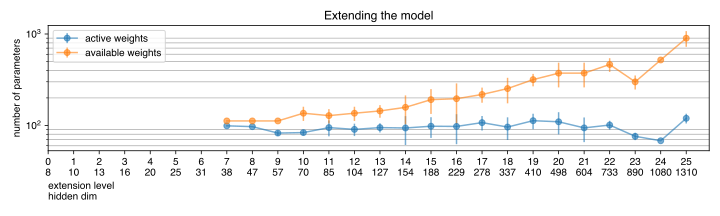
\includegraphics[width=1.0\linewidth]{extending-active-available.png}
    \caption{
        The figure depicts the number of available weights / prunable weights (orange) and the number of active weights (blue) at the iteration when the networks first split.
        Each dot represents an average over four runs with different seeds.
        The error bars indicate the standard deviation.
        While the number of available weights at the split iteration increases, the number of active weights stays fairly constant.
    }
    \label{fig:constant-active}
\end{figure}
When the network size and the number of pruning levels is increased, the networks tend to split in earlier pruning levels.
This is indicated by the number of prunable weights the network has by the time it splits.
This is depicted in figure \ref{fig:constant-active} by the organge line. 
Each point represents an average over four runs with different seeds for the model initialization. 

TODO: compare the degradation iteration and see if the same trend is there

\subsubsection{Performance of Lottery tickets}
are there differences in the performance of lottery tickets when they split?

compare 